\phantomsection\numberedsection{RF6.1 Crear Atributo}

\subsection*{Descripción}
Los usuarios pueden crear atributos personalizados para los productos, con un límite de hasta 5 atributos por cuenta.
\vspace{0.15cm}

\textbf{Pre-condición}\par
El usuario ha iniciado sesión en su cuenta en Mini PIM y no tiene la máxima cantidad de atributos de usuario creados.\par
\vspace{0.15cm}

\textbf{Post-condición}
\begin{itemize}
    \item Caso de éxito: El atributo es creado y reflejado en la base de datos y en la interfaz gráfica, asociado al usuario correspondiente.
    \item Caso mínimo: El sistema notifica al usuario el resultado de la acción crear atributo; exitosa o fallida.
\end{itemize}

\textbf{Prioridad: }
Alta
\vspace{0.15cm}

\textbf{Autor: }
Diego Sicre y Pablo Ortega.\par
\vspace{0.15cm}

\textbf{Control de cambios: }
\begin{itemize}
    \item Versión 1: Definición del caso de uso.
\end{itemize}

\numberedsubsection{Escenario principal}
\begin{enumerate}
    \item El usuario se encuentra en la sección de atributos y selecciona la opción \enquote{Añadir atributo}.
    \item El sistema despliega un formulario solicitando los siguientes datos:
    \begin{itemize}
        \item Nombre del atributo (campo obligatorio).
        \item Tipo de dato (ej. Texto, Imagen, Número Entero).
    \end{itemize}
    \item El usuario introduce los datos solicitados:
    \begin{itemize}
        \item Si selecciona Texto como tipo de dato, el sistema establece un límite de 250 caracteres para el valor.
    \end{itemize}
    \item El usuario confirma la creación del atributo.
    \item El sistema verifica que:
    \begin{itemize}
        \item El usuario no ha superado el límite de 5 atributos creados.
        \item El nombre del atributo y el tipo de dato son válidos y cumplen las restricciones establecidas.
    \end{itemize}
    \item El sistema almacena el nuevo atributo en la base de datos, asociado al usuario.
    \item El sistema muestra al usuario un mensaje confirmando que el atributo ha sido creado con éxito y lo agrega a la lista de atributos disponibles.
\end{enumerate}

\numberedsubsection{Escenarios alternativos}
\begin{description}
    \item[4.a] El sistema detecta que el usuario ha alcanzado el límite de 5 atributos creados.
    \begin{enumerate}
        \item[4.a.1] El sistema muestra un mensaje indicando que no es posible crear más atributos, ya que se ha alcanzado el límite permitido.
    \end{enumerate}
\end{description}

\numberedsubsection{Casos de Prueba}
\underline{Escenario: Principal}\par
\vspace{0.15cm}
\textbf{Dado} que el usuario ha iniciado sesión en su cuenta en Mini PIM,\par
\textbf{Y} se encuentra en la sección de atributos,\par
\textbf{Cuando} selecciona la opción de \enquote{Añadir atributo},\par
\textbf{E} introduce un nombre y selecciona un tipo de dato válido,\par
\textbf{Y} confirma la creación,\par
\textbf{Entonces} el sistema almacena el nuevo atributo en la base de datos y lo muestra en la lista de atributos disponibles.\par
\vspace{0.20cm}

\underline{Escenario: Alternativo 2.a}\par
\vspace{0.15cm}
\textbf{Dado} que el usuario ha iniciado sesión en su cuenta en Mini PIM,\par
\textbf{Y} se encuentra en la sección de atributos,\par
\textbf{E} intenta seleccionar un tipo de dato no soportado,\par
\textbf{Cuando} confirma la creación del atributo,\par
\textbf{Entonces} el sistema muestra un mensaje de error y permite al usuario corregir la selección del tipo de dato.\par
\vspace{0.20cm}

\underline{Escenario: Alternativo 4.a}\par
\vspace{0.15cm}
\textbf{Dado} que el usuario ha iniciado sesión en su cuenta en Mini PIM,\par
\textbf{Y} se encuentra en la sección de atributos,\par
\textbf{Y} que el usuario ya ha creado 5 atributos,\par
\textbf{Cuando} intenta crear uno nuevo,\par
\textbf{Entonces} el sistema notifica que se ha alcanzado el límite de atributos permitidos y no permite la creación.\par
\vspace{0.20cm}

\underline{Escenario: Alternativo 5.a}\par
\vspace{0.15cm}
\textbf{Dado} que el usuario ha iniciado sesión en su cuenta en Mini PIM,\par
\textbf{Y} se encuentra en la sección de atributos,\par
\textbf{Y} que el usuario hay un error en el nombre del atributo,\par
\textbf{Cuando} intenta confirmar la creación,\par
\textbf{Entonces} el sistema muestra un mensaje de error indicando el campo faltante y permite al usuario corregirlo.\par
\vspace{0.20cm}


\numberedsubsection{Bocetos}
\begin{figure}[H]
    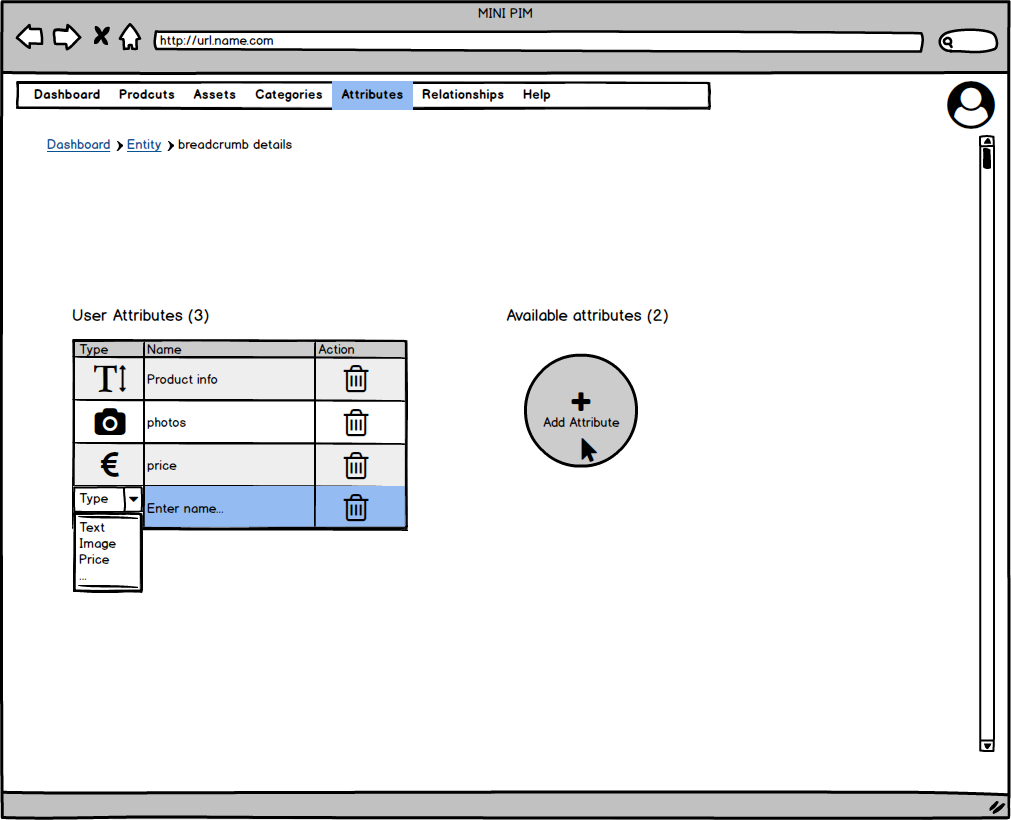
\includegraphics[width=1\linewidth]{mockups/RF6.1Crear_Atributo tras Clickar.png}
    \caption{Menú de creación tras clicar \enquote{Añadir atributo}}
   \end{figure}
\vspace{1.0cm}

\newpage %Inicia en una nueva página otro caso de uso